\section{Umsetzung:}
\subsection*{HomeScreen:}
\begin{figure}[h!]
    \begin{minipage}[c]{0.5\textwidth}
      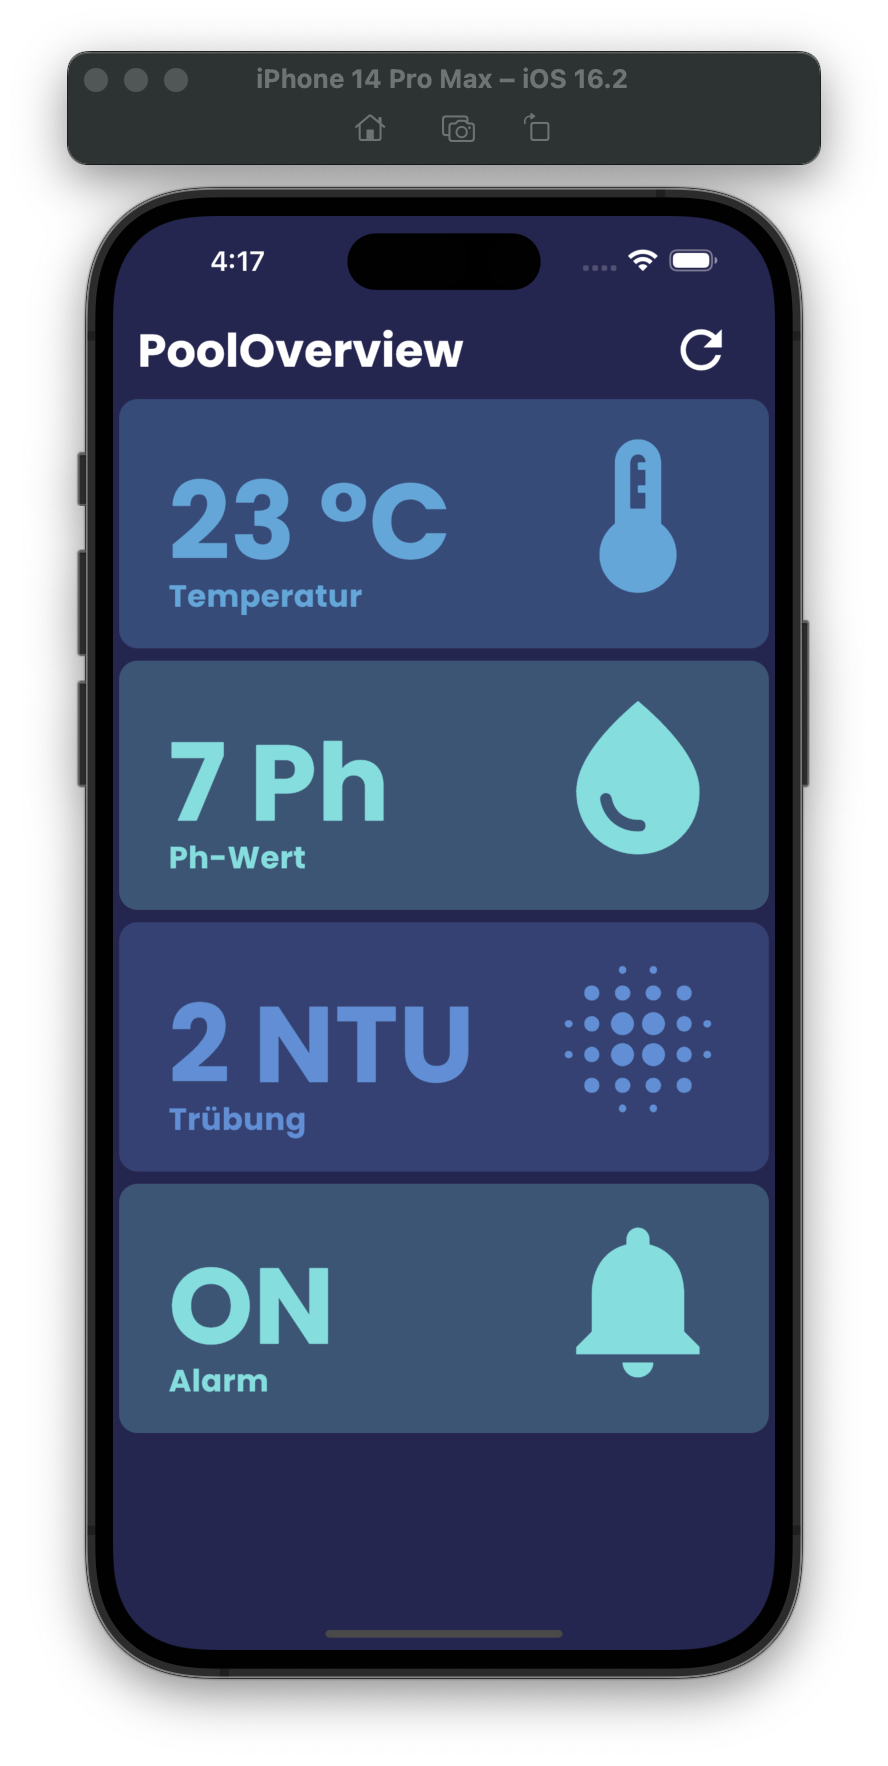
\includegraphics[width=\textwidth]{./pics/StartpageBild.png}
    \end{minipage}
    \begin{minipage}[c]{0.5\textwidth}
      \label{fig:deinbild}
      Der Home-Screen basiert auf einem Scroll-View,
      welches den Vorteil bietet ein einheitliches Design auf jeder Art von Bildschrimgröße zu gewährleisten, ohne die Lesbarkeit zu beeinträchtigen. 
      Ein ScrollView in Flutter ist ein Widget, das verwendet wird, um eine Liste von Elementen anzuzeigen, die größer sind als der verfügbare Bildschirm. 
      Es ermöglicht dem Benutzer, durch die Liste zu scrollen, um alle Elemente anzuzeigen. Es gibt verschiedene Arten von ScrollView in Flutter, darunter ScrollView, ListView, GridView und CustomScrollView. Das ScrollView enthält generisch selbst erstellte Objekte names DataCard.
    \end{minipage}
  \end{figure}
  \newpage
  \subsection*{DataCards:}
  \begin{figure}[h!]
    \begin{minipage}[c]{0.5\textwidth}
      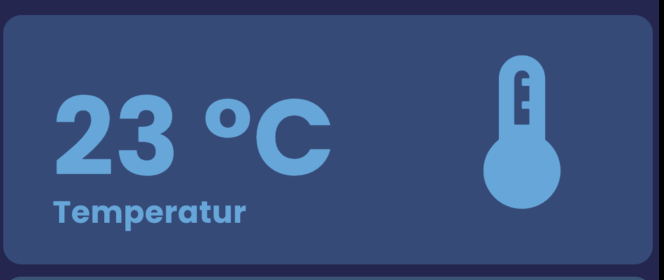
\includegraphics[width=\textwidth]{./pics/Bildschirm­foto 2023-03-24 um 16.25.49.png}
    \end{minipage}
    \begin{minipage}[c]{0.5\textwidth}
      \label{fig:DataCard}
      Das DataCard Widget in Flutter ist ein vorgefertigtes Material Design-Widget, das zur Darstellung von Informationen in einem Kartenformat verwendet wird. 
      Es besteht aus einer rechteckigen Box mit abgerundeten Ecken, die in der Regel eine Hintergrundfarbe, einen Titel, eine Beschreibung und optional eine Aktion oder einen Button enthält.
      Das DataCard Widget enthält verschiedene Eigenschaften, die angepasst werden können, um das Erscheinungsbild und das Verhalten der Karte zu steuern. Dazu gehören Eigenschaften wie Hintergrundfarbe, Ränder, Schatten, Größe, Padding und Ausrichtung.  
    \end{minipage}
  \end{figure}
DataCards verfügen über die Funktion „onPressed“ in der man angeben kann was geschieht, wenn man eine der 5 DataCards drückt. Wenn man eine DataCard die den Namen „Temperatur“, „Ph-Wert“ oder „Trübung“ drückt wird man an eine weitere Page der App weiter geleitet in der man Statistiken zu dem jeweiligen Wert erhält. Wenn man die DataCard mit dem Namen „Alarm“ drückt wird der Alarm den man erhält wenn verdächtige Bewegungen des Gyroskopssensors wahrgenommen werden aktiviert oder deaktiviert.
Die DataCards auf dem HomeScreen enthalten ansonsten den zuletzt gemessenen Wert, der durch einen WebSocket vom Backend bereitgestellt wird und stellen diesen dar. Die DataCards sind generisch erstellbar mit Übergabewerten, was eine einfache Vergrößerung des Funktionsumfangs des HomeScreens ermöglicht.
Die Icons die auf den DataCards zu sehen sind, werden von Google-Material-Icons bereitgestellt und werden mittels API in die App Ressourceneffizient implementiert.
\begin{figure}[h!]
    \begin{minipage}[c]{0.5\textwidth}
      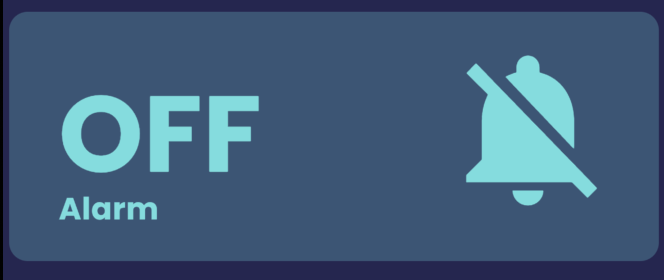
\includegraphics[width=\textwidth]{./pics/Bildschirm­foto 2023-03-24 um 16.22.40.png}
    \end{minipage}
    \begin{minipage}[c]{0.5\textwidth}
      \label{fig:AlarmOFF}
      So sieht die DataCard aus wenn man den Alarm durch drücken des Feldes deaktivert.
    \end{minipage}
\end{figure}
\newpage
\subsection*{Grafische Darstellung der Werte über Zeit:}

\begin{figure}[h!]
    \begin{minipage}[c]{0.4\textwidth}
      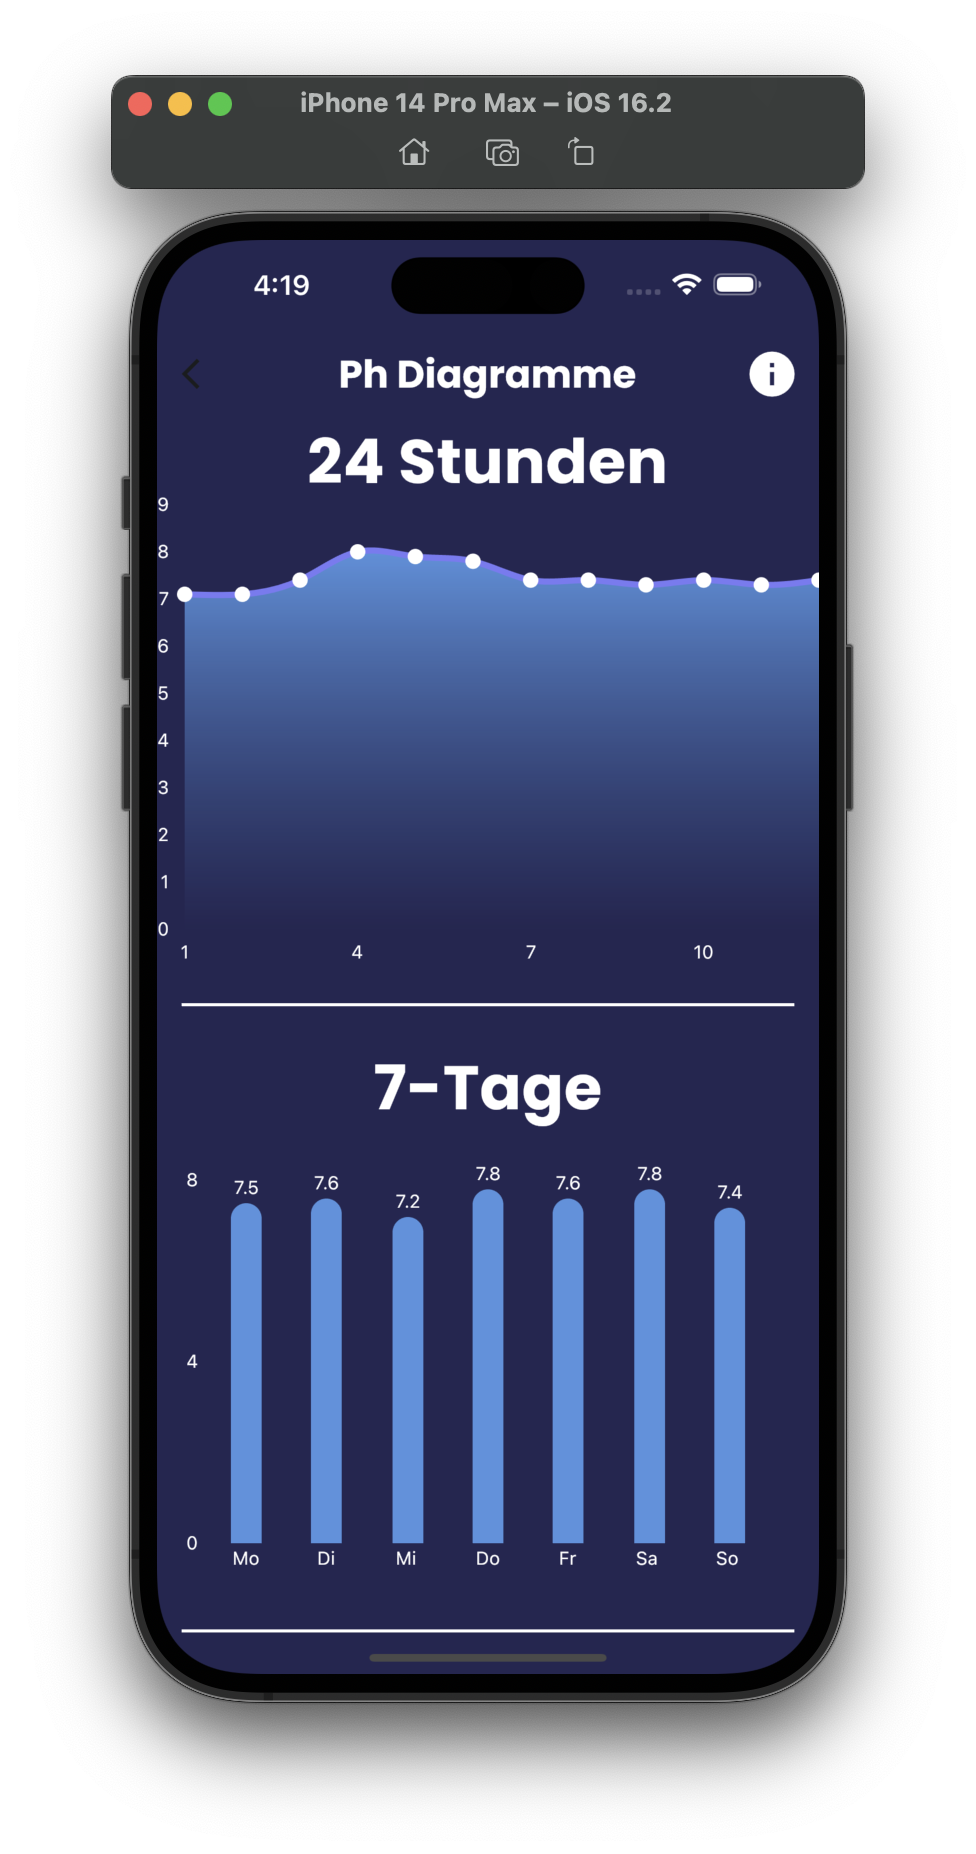
\includegraphics[width=\textwidth]{./pics/Diagramme1Bild.png}
    \end{minipage}
    \begin{minipage}[c]{0.5\textwidth}
      \label{fig:DigrammeApp1}
      Hier sind die Diagramme dargestellt auf die man durch das klicken der DataCards weiter geleitet wird. 
      Sie werden durch die Libraries "charts\_flutter" und "syncfusion\_flutter\_charts" bereitgestellt und mittels
      HTTP-Request befüllt und bei aufruf aktualisiert.

    \end{minipage}
\end{figure}
\begin{figure}[h!]
    \begin{minipage}[c]{0.4\textwidth}
      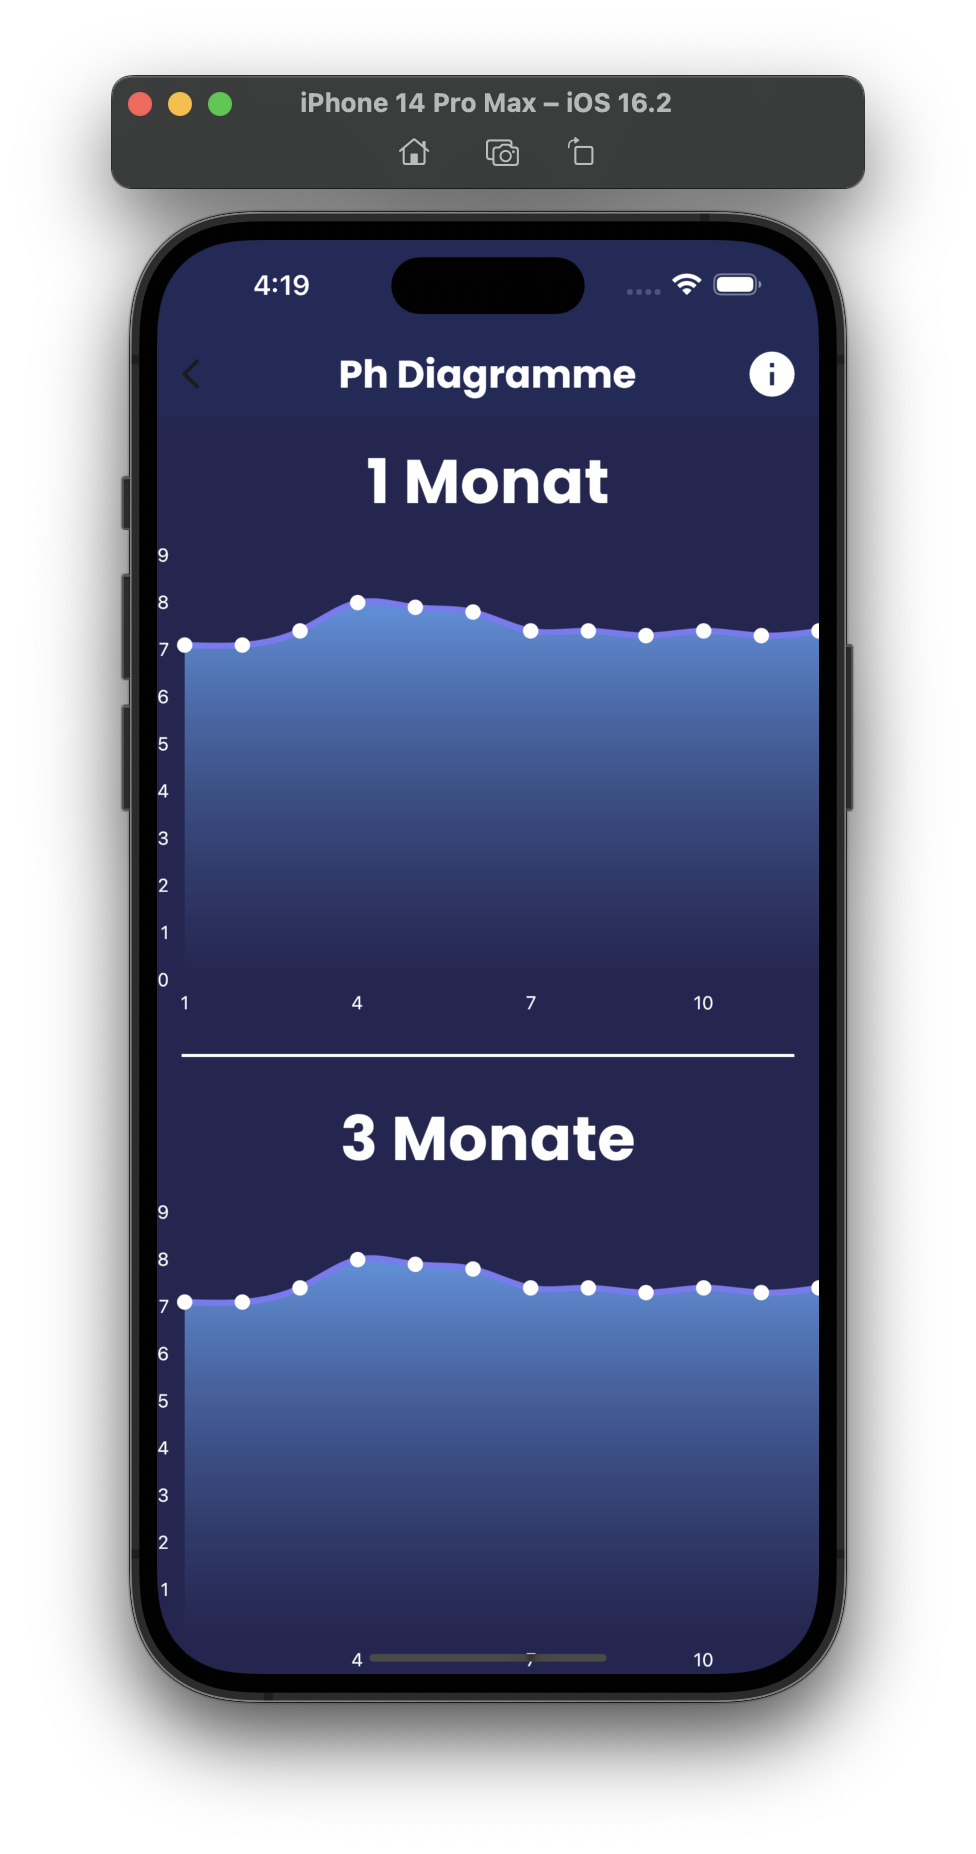
\includegraphics[width=\textwidth]{./pics/Diagramme2Bild.png}
    \end{minipage}
    \begin{minipage}[c]{0.5\textwidth}
      \label{fig:DiagrammeApp2}
      Nach dem Freunde Verwandte und Bekannte mittels mündlicher Umfrage befragt wurden, ist beschlossen worden, dass
      Diagramme in den Zeiträumen "24 Stunden", "7 Tage", "1 Monat" und "3Monate" angezeigt werden sollen.
      Diese Zeiträume waren am beliebtesten und sind wenn man die durchschnittliche Dauer einer Badesaison betrachtet am relevantesten
      für den Benutzer dieser Applikation.
    \end{minipage}
\end{figure}
\newpage

\subsection*{Designkonzept:}
Bei dem Design wurde ein sehr schlichtes und leicht zuverstehedes Material-Design gewählt.
Es basiert auf der Schriftart "Poppins-Bold" und macht die App sehr anschaulich. Die Graphen werden bei Aufruf
dynamisch mit den Daten aus der Datenbank befüllt und aktualisiert und dieser Ablauf durch eine Animation in der sich der Graph langsam aufbaut
überbrückt. Die verwendeten Icons werden von Google-Material-Icons bereitgestellt und sind nach belieben veränderbar.
Das Design ist dynamisch und passt sich jeder Bildschrimgröße, Auflösung und Bildschirmverhältnis an.
\begin{figure}[h!]
\begin{minipage}[c]{0.5\textwidth}
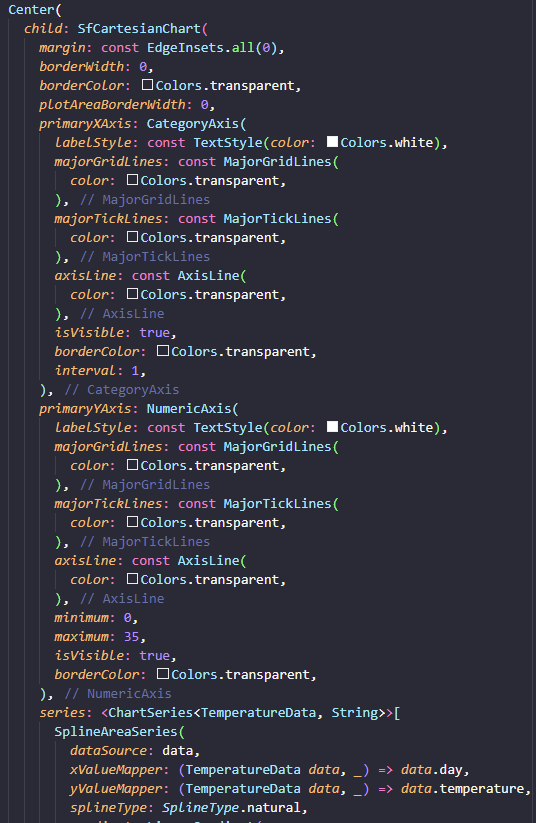
\includegraphics[width=\textwidth]{./pics/CodeSnippetChartDesign.PNG}
\end{minipage}
\begin{minipage}[c]{0.5\textwidth}
    \label{fig:CodeSnippetGraph}
    Dieses Code-Snippet zeigt einen kleinen Einblick wie man einen Graphen designed und mit seinen dazugehörigen 
    Daten befüllt. Ein Graph braucht eine bestimtme Art von Liste durch die er befüllt wird. Die Daten 
    die sich in dieser Liste befinden werde vorher von der Logik durch die HTTP-Request abgefragt und für jeden Graphen einzeln
    aufbereitet um die Daten anschaulich darzustellen.
\end{minipage}
\end{figure}
\newline 
Da der die Sinus-Grpahen jedem Tag nur einen druchschnitts Wert zuordnen um somit die Darstellung übersichtlicher
zu gestalten wird davor für jeden Tag ein Durschnittswert berechnet. Da das Backend um Bits zu sparen nur einen Epoch-Timestamp übergibt
muss dies auch vorher aufbereitet werden.




